\subsection{BER bounds for Raptor codes in Rayleigh fading channels}
\cri{Qui sottolinea che il odo di procedere nella dimostrazione è uguale a dopo}
The last notable result we focus on is depicted in \cite{Yue2013} where Yue \textit{et al.} derive a lower bound for the LT-based \gls{dnc} scheme over Rayleigh fading channels and upper/lower bounds for the \gls{ber} in the Raptor based version, in which an inner LT code concatenates a conventional outer code to reduce the error floor.

The scenario of the paper provides a \gls{wsn} with multiple source and relay nodes and a single sink. The main difference with the scenario depicted in \autoref{sec:relayBER} is that here the relay nodes must be of two types: a precoding relay group and an LT-coding relay group. Finally, in this case the decoding is performed throught the \gls{ml} criterium.

\subsubsection{Lower BER bound for LT scheme}
In \cite{Yue2013} the authors first find a lower bound for the LT-based \gls{dnc} scheme with \gls{ml} decoding over Rayleigh fading channel, starting from the information sequence error probability
\begin{equation}
  P_e = P_r\biggl(\bigcup\limits_{\mathbf{e}:\omega(\mathbf{e})\neq 0}\hat{\mathbf{m} }= \mathbf{e}\biggr)
\end{equation}
In this case, $\hat{\mathbf{m}}$ is the estimated information sequence and $\omega(\cdot)$ the Hamming weight as usual. This probability is given by the probability that only one symbol in the decoded sequence is recovered uncorrectly. Inside this value, the part representing the Rayleigh fading channel is given by $P_r(\mathbf{v}\rightarrow \mathbf{v}'|\hbar)$, which is the conditional probability that the decoded codeword is equal to $\mathbf{v}'$ give the channel fading coefficient $\hbar$.

For what concerns the bounds on \gls{ber} for Raptor codes we can see that:
\begin{itemize}
  \item The probability of decoding errors for a Raptor code of parameters $\Omega(x)$, $\mu(x)$, $K_L$, $K$, $Q$ and expanding coefficient $\eta$ is upperbounded by $P_b < \min\{1,\xi_U^{Raptor}\}$, with $\xi_U^{Raptor}$ given by:
  \begin{equation}
    \xi_U^{Raptor} = \sum_{t=1}^K\frac{1}{K}\binom{K}{t}\xi_U^t(1-\xi_U)^{K-t}\cdot\Bigl(\sum_{\omega(\mathbf{h})}\Omega_{\omega(\mathbf{h})}\zeta_t^{R,\omega(\mathbf{h})}\Bigr)^{K-K_L}
  \end{equation}
  where
  \begin{equation}
    \zeta_t^{R,\omega(\mathbf{h})} = \frac{\sum_{\alpha = even,0\leq\alpha\leq t}\binom{t}{\alpha}\binom{K-t}{\omega(\mathbf{h})-\alpha}}{\binom{K}{\omega(\mathbf{h})}}
  \end{equation}
  \item The probabilty of the aforementioned Raptor code is lower bounded by $P_b > \max\{0,\xi_L^{Raptor}\}$, where $\xi_L^{Raptor}$ is given by:
  \begin{align}
    &\xi_L^{Raptor} = \sum_{t=1}^K\frac{1}{K}\binom{K}{t}\xi_L^t(1-\xi_L)^{K-t}\Bigl(\sum_{\omega(\mathbf{h})}\Omega_{\omega(\mathbf{h})}\zeta_t^{R,\omega(\mathbf{h})}\Bigr)^{K-K_L}-\frac{1}{2}\sum_{t=1}^K\binom{K}{t}\times\\
    &\xi_U^t(1-\xi_U)^{K-t}\sum_{\tau_0}^t\sum_{\tau_1 = t-\tau_0}\sum_{\tau_2=0}^{K-\tau_0}\frac{\binom{t}{\tau_0}}{2^t}\frac{\binom{K-\tau_0}{\tau_2}}{2^{K-\tau_0}}\frac{\binom{K-\tau_0}{\tau_2}}{2^{K-\tau_0}}\Bigl(\sum_{\omega(\mathbf{h})}\Omega_{\omega(\mathbf{h})}\zeta(\tau_0,\tau_1,\tau_2,t)\Bigr)^{K-K_L}
  \end{align}
  where
  \begin{equation}
    \zeta_t^{R,\omega(\mathbf{h})} = \frac{\sum\limits_{\alpha = even,0\leq\alpha\leq t}\binom{t}{\alpha}\binom{K-t}{\omega(\mathbf{h})-\alpha}}{\binom{K}{\omega(\mathbf{h})}} = \frac{\sum\limits_{\alpha=even,0\leq\alpha\leq \min\{\tau_p,\omega(\mathbf{h_{\tau_p}})\}}\binom{\tau_p}{\alpha}\binom{K-\tau_p}{\omega(\mathbf{h})-\alpha}}{\binom{K}{\omega(\mathbf{h})}}
  \end{equation}
\end{itemize}
Moreover, we specify that $\xi_U$ is the upper \gls{ber} bound of the LT codes, while $\mathbf{h}$ is a column vector of the parity check matrix $\mathbf{H}$ and that $\tau_i$ is the length of the $i^{th}$ of its columns. We refer to \cite{Yue2013} for the proof, which, moreover, is designed with the same structure as the one of the BER bounds for LT-codes in \cite{Yue2014}.
\subsubsection{Results}
The results in \cite{Yue2013} show several important points: first of all, that both the LT codes and the Raptor codes \gls{ber} bounds become asymptotically tight to one another as the expanding coefficient $\eta$ grows. Furthermore, as shown in figure \autoref{fig:BEReta}, the performance of Raptor codes are much better than LT-codes, regardless of the expanding coefficient. This behavior is coherent with the results that Yue \textit{et al.} also find in \cite{Yue2014}.

It is also shown that there is an enhancement with respect to the value of $E_s/N_0$ since, as it increases, the difference $\xi_U^{Raptor}-\xi_L^{Raptor}$ becomes smaller; and finally that as the code rate of the codes used in the construction of the Raptor codes decreases, the \gls{ber} bounds get better.
\begin{SCfigure}
  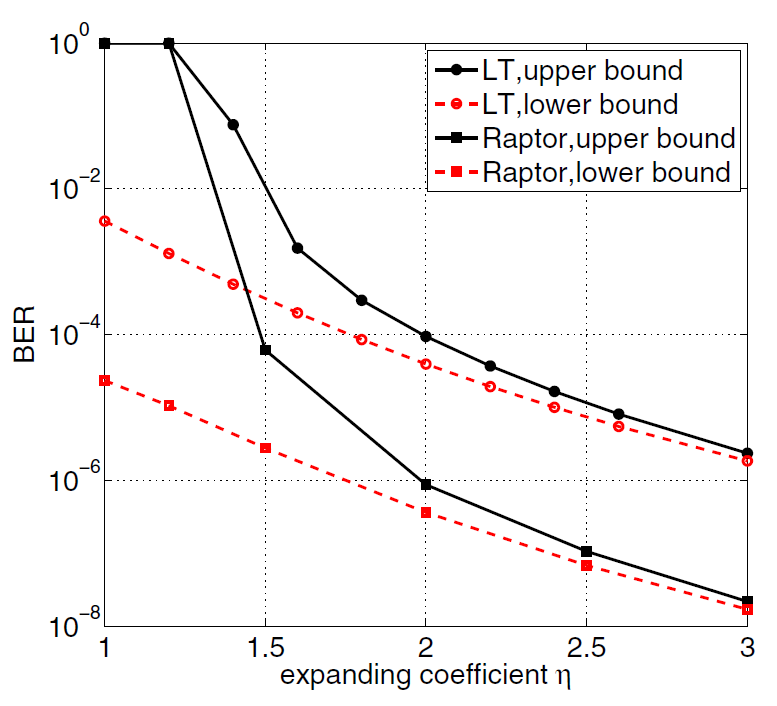
\includegraphics[width = 0.45\textwidth]{bounds_3.png}
  \caption{\gls{ber} bounds comparison for LT-based and Raptor-based \gls{dnc} schemes over Rayleigh fading channels with $K_L = 98$, $K = 100$ and $E_s/N_0 = 7dB$. Source \cite{Yue2013}}
  \label{fig:BEReta}
\end{SCfigure}
